\documentclass[12pt, twoside]{article}
\usepackage[utf8]{inputenc}
\usepackage[english,russian]{babel}

\usepackage{amsthm}

\usepackage{graphicx}
\usepackage{caption}
\usepackage{amssymb}
\usepackage{amsmath}
\usepackage{mathrsfs}
\usepackage{euscript}
\usepackage{graphicx}
\usepackage{subfig}
\usepackage{caption}
\usepackage{color}
\usepackage{bm}
\usepackage{tabularx}
\usepackage{adjustbox}


\usepackage[toc,page]{appendix}

\usepackage{comment}
\usepackage{rotating}

\DeclareMathOperator*{\argmax}{arg\,max}
\DeclareMathOperator*{\argmin}{arg\,min}

\newtheorem{theorem}{Теорема}
\newtheorem{lemma}[theorem]{Лемма}
\newtheorem{definition}{Определение}[section]

\numberwithin{equation}{section}

\newcommand*{\No}{No.}
\begin{document}

\begin{comment}
\title{\bf Attention для апроксимации временных рядов}
\end{comment}
\title{\bf Анализ свойств локальных моделей в задачах кластеризации временных рядов\thanks{Работа выполнена при поддержке РФФИ и правительства РФ.}}
\date{}
\author{}
\maketitle

\begin{center}
\bf
А.\,В.~Грабовой\footnote{Московский физико-технический институт, grabovoy.av@phystech.edu}, В.\,В.~Стрижов\footnote{Вычислительный центр им. А.~А. Дородницына	ФИЦ ИУ РАН, strijov@ccas.ru}

\end{center}

{\centering\begin{quote}
\textbf{Аннотация:} Данная работа посвящена поиску периодических сигналов во временных рядах с целью распознавания физических действий человека с помощью акселерометра. Предлагается метод кластеризации точек временного ряда для поиска характерных периодических сигналов внутри временного ряда. Для построения признакового описания используется метода главных компонент для локального снижения размерности фазового пространства. Для оценки близости двух периодических сигналов вычисляется расстояние между базисными векторами, которые получены методом главных компонент. Используя матрицу попарных расстояний между точками временного ряда выполняется кластеризация данных точек. Для анализа качества представленного алгоритма проводятся эксперименты на синтетических данных и данных полученных при помощи мобильного акселерометра.


\smallskip
\textbf{Ключевые слова}: временные ряды; кластеризация; распознание физической активности; метод главных компонент.

\smallskip
\textbf{DOI}: 00.00000/00000000000000
\end{quote}
}

\section{Введение}
Анализ физической активности человека производится при помощи мобильных телефонов, разумных часов. Эти устройства используют акселерометр, гироскоп и магнитометр. Цель данной работы заключается в  разметке b распознавании человеческой активности во времени. %Некоторые сходства с данной задачей можно увидеть в работах по классификации временных рядов~\cite{Ignatov2015}, а также задача об обнаружении периодов активности~\cite{Olivares2012, cinar2018}.

Временные ряды~---~это объекты сложной структуры, при классификации которых значимую роль играет метод построения признакового пространства. Для этой цели используются: экспертно заданные базовые функций, гипотеза порождения данных. В \cite{Ivkin2015} рассматривается комбинированное признаковое описание на основе данных методов. В \cite{Katrutsa2015} также рассматривается проблема построение признакового пространства и предлагается критерий избыточности выбранных признаков.
\begin{figure}[h!t]\center
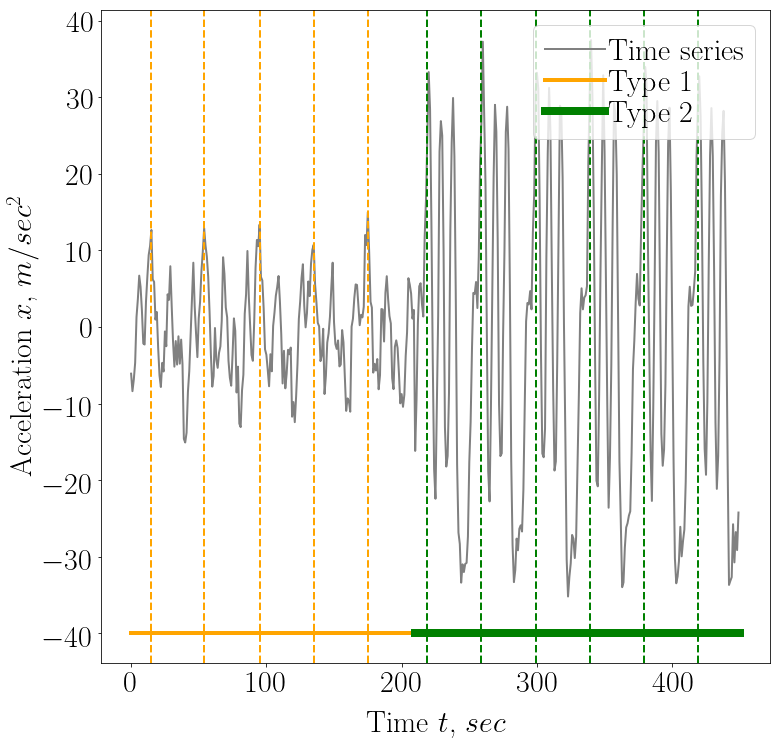
\includegraphics[width=1\textwidth]{results/example}\\
\caption{Временной ряд, с разметкой на кластеры.}
\label{example_1}
\end{figure}

В данной работе решается задача кластеризации точек временного ряда. При \textit{кластеризации} каждой точке временного ряда ставится в соответствие некоторая метка. Она соответствует сегменту временного ряда. \textit{Сегмент} временного ряда это часть временного ряда, которая соответсвует одному характерному физическому действию, которое является переодическим, например: один шаг, двумя ногами при ходьбе, или один шаг, двумя ногами при беге. Пример сегментации показан на  рис.~\ref{example_1}. Также показан пример кластеризации временного ряда. Ряд, полученный при помощи акселерометра, разбит на два характерных физических действия.

Решение задачи кластеризации состоит из двух этапов. Во-первых для получения признакового описания временного ряда предлагается алгоритм локальной аппроксимации временного ряда при помощи метода главных компонент~\cite{Shiglavsi1997}. Под \textit{локальной} аппроксимацией временного ряда подразумевается, что для признакового описания его точки используется не весь ряд, а только некоторая окрестность данной точки. Во-вторых рассматривается метрика в новом пространстве признакового описания. После получения расстояния между точками временного ряда используется метод кластеризации KMeans~\cite{Kanungo2000} для кластеризации точек временного ряда.

Для решения задачи кластеризации точек временного ряда вводится предположения. Предполагается, что периоды различных сегментов различаются незначительно, причем известны минимальный и максимальный периоды сегмента и количество различных сегментов внутри временного ряда. Также предполагается, что тип активности во времени не меняется часто, а также что фазовые траектории разных сегментов являются различными. 

Проверка и анализ метода проводится на синтетической и реальной выборках. Синтетическая выборка построенная при помощи суммы нескольких первых членов ряда Фурье со случайными коэффициентами. Реальные данные получены при помощи мобильного акселерометра, который снимал показания во время некоторой физической активности человека.



\section{Постановка}

Задан временной ряд:
\begin{equation}
\label{eq:st:1}
\begin{aligned}
\textbf{x} \in \mathbb{R}^{N},
\end{aligned}
\end{equation}
где $N$ количество точек, которыми задается временной ряд.

Пусть временной ряд состоит из последовательности сигналов из множества $\mathbf{V}$:
\begin{equation}
\label{eq:st:2}
\begin{aligned}
\textbf{x} = [\textbf{v}_1, \textbf{v}_2, \cdots, \textbf{v}_M],
\end{aligned}
\end{equation}
где $\textbf{v}_i$ некоторый сигнал из множества возможных сигналов $\mathbf{V}$. Причем $\forall i$ выполняется или $\textbf{v}_i = \textbf{v}_{i-1}$ или   $\textbf{v}_i = \textbf{v}_{i+1}$. Пусть множество $\mathbf{V}$ удовлетворяет следующим свойствам:

\begin{equation}
\label{eq:st:3}
\begin{aligned}
\left|\mathbf{V}\right| = K, \quad \forall \textbf{v} \in \mathbf{V}~\left|\textbf{v}\right| \leq T,
\end{aligned}
\end{equation}
где $\left|\mathbf{V}\right|$ мощность множества сигналов, а $\left|\textbf{v}\right|$ длина сигнала.

Рассмотрим отображение:
\begin{equation}
\label{eq:st:4}
\begin{aligned}
a : x \to \{1,\cdots, K\}, 
\end{aligned}
\end{equation}
где $x \in \textbf{x}$ некоторая точка временного ряда.

Требуется, чтобы отображение удовлетворяло следующим свойствам:

\begin{equation}
\label{eq:st:5}
\begin{aligned}
\begin{cases}
    a\left(x_1\right) = a\left(x_2\right), & \text{если найдется}~\textbf{v} \in \mathbf{V}: x_1,x_2 \in \textbf{v}\\
    a\left(x_1\right) \not= a\left(x_2\right), & \text{если не найдется}~\textbf{v} \in \mathbf{V}: x_1,x_2 \in \textbf{v}
\end{cases}
\end{aligned}
\end{equation}

Пусть задана некоторая асессорская разметка временного ряда:
\begin{equation}
\label{eq:st:6}
\begin{aligned}
\textbf{y} \in \{1,\cdots,K\}^{N}.
\end{aligned}
\end{equation}

Тогда ошибка, которую совершает алгоритм $a$ на временном ряде $\textbf{x}$ представляется в следующем виде:
\begin{equation}
\label{eq:st:7}
\begin{aligned}
S = \frac{1}{N}\sum_{i=1}^{N}[y_i = a\left(x_i\right)],
\end{aligned}
\end{equation}
где $x_i$ --- точки временного ряда,  $y_i$ асессорская разметка временного ряда.

\section{Кластеризация точек}
Рассматривается фазовая траектория временного ряда $\textbf{x}$:
\begin{equation}
\label{eq:cl:1}
\begin{aligned}
\mathbf{H} = \{\textbf{h}_t| \textbf{h}_t = [x_{t-T}, x_{t-T+1}, \cdots, x_{t}],~T\leq t\leq N\}.
\end{aligned}
\end{equation}

Фазовая траектория разбивается на фазовые подпространства из $2T$ векторов:
\begin{equation}
\label{eq:cl:2}
\begin{aligned}
\mathbf{S} = \{\textbf{s}_t| \textbf{s}_t = [h_{t-T}, h_{t-T+1}, \cdots, h_{t+T-1}],~T\leq t\leq N-T\},
\end{aligned}
\end{equation}
полученное подпространство имеет всю локальную информацию об временном ряде, так-как содержит всю информацию на периоде до момента времени $t$ и информацию на периоде после момента времени $t$.

Каждое $T\text{-мерное }$ подпространство $\textbf{s}_t$ проектируется на подпространство значительно меньшей размерности при помощи метода главных  компонент~$\textbf{z}_t~=~\textbf{W}_t\textbf{s}_t$. Получим представление базисных векторов $\textbf{W}_t$, а также собственные числа, которые соответствуют данным базисным векторам каждого подпространства $\textbf{s}_t$ в $T\text{-мерном}$ пространстве:
\begin{equation}
\label{eq:cl:3}
\begin{aligned}
\mathbf{W} = \{\textbf{W}_t| \textbf{W}_t = [\textbf{w}^1_t, \textbf{w}^2_t]\}, \quad \bm{\Lambda} = \{\bm{\lambda}_t| \bm{\lambda}_t=[\lambda^1_t, \lambda^2_t]\},
\end{aligned}
\end{equation}
где $[\textbf{w}^1_t, \textbf{w}^2_t]$ и $[\lambda^1_t, \lambda^2_t]$ это базисные векторы и соответствующие им собственные числа плоскости построенной при помощи метода главных компонент для подпространстве $\textbf{s}_t$.

Рассмотрим функцию расстояние между элементами $\mathbf{W}$:
\begin{equation}
\label{eq:cl:4}
\begin{aligned}
\rho\left(\textbf{W}_1, \textbf{W}_2\right) = \max\left(\max_{\textbf{e}_2 \in \textbf{W}_2} h_{1}\left(\textbf{e}_2\right), \max_{\textbf{e}_1 \in \textbf{W}_1} h_{2}\left(\textbf{e}_1\right)\right),
\end{aligned}
\end{equation}
где  $\textbf{e}_i$ это базисный вектор пространства $\textbf{W}_i$, $h_i\left(\textbf{e}\right)$ является расстоянием от вектора $\textbf{e}$ до пространства $\textbf{W}_i$.

Функция расстояния~(\ref{eq:cl:4}) является метрикой, доказательство этого факта представлено в приложении \ref{ProofTheorem1}. В случае, когда подпространства $\textbf{W}_t$ имеет размерность два, тогда $\rho\left(\textbf{W}_1, \textbf{W}_2\right)$ имеет следующую интерпретацию:

\begin{equation}
\label{eq:cl:5}
\begin{aligned}
\rho\left(\textbf{W}_1, \textbf{W}_2\right) = \max_{\{\textbf{a},\textbf{b},\textbf{c}\} \subset \textbf{W}_1\cup \textbf{W}_2 } V\left(\textbf{a},\textbf{b},\textbf{c}\right), 
\end{aligned}
\end{equation}
где $V\left(\textbf{a},\textbf{b},\textbf{c}\right)$ --- объем параллелепипеда построенного на векторах $\textbf{a}, \textbf{b}, \textbf{c}$, которые являются базисными векторами.


Рассмотрим расстояние между элементами $\bm{\Lambda}$:
\begin{equation}
\label{eq:cl:6}
\begin{aligned}
\rho\left(\bm{\lambda}_1, \bm{\lambda}_2\right) = \sqrt[]{\left(\bm{\lambda}_1 - \bm{\lambda}_2\right)^{\mathsf{T}}\left(\bm{\lambda}_1 - \bm{\lambda}_2\right)}.
\end{aligned}
\end{equation}

$\rho\left(\bm{\lambda}_1, \bm{\lambda}_2\right)$ является метрикой в пространстве $\mathcal{L}$.

Матрица попарных расстояний между базисными векторами для временного ряда $\textbf{x}$:
\begin{equation}
\label{eq:cl:7}
\begin{aligned}
\textbf{M}_{\text{c}} = [0, 1]^{N\times N}.
\end{aligned}
\end{equation}

Матрица попарных расстояний между собственными значениями для временного ряда $\textbf{x}$:
\begin{equation}
\label{eq:cl:8}
\begin{aligned}
\textbf{M}_{\text{l}} = [0, 1]^{N\times N}.
\end{aligned}
\end{equation}

Используя выражения~(\ref{eq:cl:5}-\ref{eq:cl:8}) определим расстояние между двумя точками $t_1, t_2$ временного ряда:
\begin{equation}
\label{eq:cl:9}
\begin{aligned}
\rho\left(t_1, t_2\right) = \rho\left(\textbf{W}_1, \textbf{W}_2\right) + \rho\left(\bm{\lambda}_1, \bm{\lambda}_2\right), \quad \textbf{M} = \textbf{M}_{\text{l}} + \textbf{M}_{\text{c}},
\end{aligned}
\end{equation}
где $\rho\left(t_1, t_2\right)$ является метрикой, так-как является суммой двух метрик. Матрица $\textbf{M}$ является матрицей попарных расстояний между двумя точками временного ряда.

Используя матрицу попарных расстояний $\textbf{M}$ выполним кластеризацию моментов времени временного ряда, получим следующее отображение:

\begin{equation}
\label{eq:cl:10}
\begin{aligned}
a : x \to \{1,\cdots, K\}, 
\end{aligned}
\end{equation}
где $x$ некоторая точка временного ряда \textbf{x}.


\section{Эксперимент}
Для анализа свойств предложенного алгоритма был проведен вычислительный эксперимент в котором кластеризация точек временного ряда проводилась используя матрицы попарных расстояний ~$(\ref{eq:cl:9})$.

В качестве данных использовались две выборки временных рядов, которые описаны в таблице~\ref{table_1}. Выборка Physical Motion это реальные временные ряды полученные при помощи мобильного акселерометра. Синтетические временные ряды были построены при помощи нескольких первых слагаемых ряда Фурье со случайными коэффициентами из стандартного нормального распределения. Генерация данных состояла из двух этапов. На первом этапе генерировались короткие сигналы $\textbf{v}$ для построения множества $\mathbf{V}$. Вторым этапом генерации выборки $\textbf{x}$ является следующим случайным процессом:
\begin{equation}
\label{eq:exp:1}
\begin{aligned}
\textbf{x} = [\textbf{v}_{1}, \textbf{v}_{2}, \cdots, \textbf{v}_{M}], \quad \begin{cases}
    \textbf{v}_{1} \sim \mathcal{U}\left(\mathbf{V}\right),\\
    \textbf{v}_{i} = \textbf{v}_{i - 1}, & \text{с вероятностью}~\frac{3}{4}\\
    \textbf{v}_{i} \sim \mathcal{U}\left(\mathbf{V}\right), & \text{с вероятностью}~\frac{1}{4}
\end{cases},
\end{aligned}
\end{equation}
где $\mathcal{U}\left(\mathbf{V}\right)$ --- равномерное распределение на объектах из $\mathbf{V}$.

\begin{table}[h!t]
\begin{center}
\caption{Описание выборок}
\label{table_1}
\begin{tabular}{|c|c|c|c|}
\hline
	Ряд & $N$& $K$& $T$\\
	\hline
	\multicolumn{1}{|l|}{Physical Motion 1}
	& 900& 2& 30\\
	\hline
	\multicolumn{1}{|l|}{Physical Motion 2}
	& 1000& 2& 30\\
	\hline
	\multicolumn{1}{|l|}{Synthetic 1}
	& 2000& 2& 20\\
	\hline
	\multicolumn{1}{|l|}{Synthetic 2}
	& 2000& 3& 20\\
\hline

\end{tabular}
\end{center}
\end{table}

\begin{figure}[h!t]\center
\subfloat[Synthetic 1]
{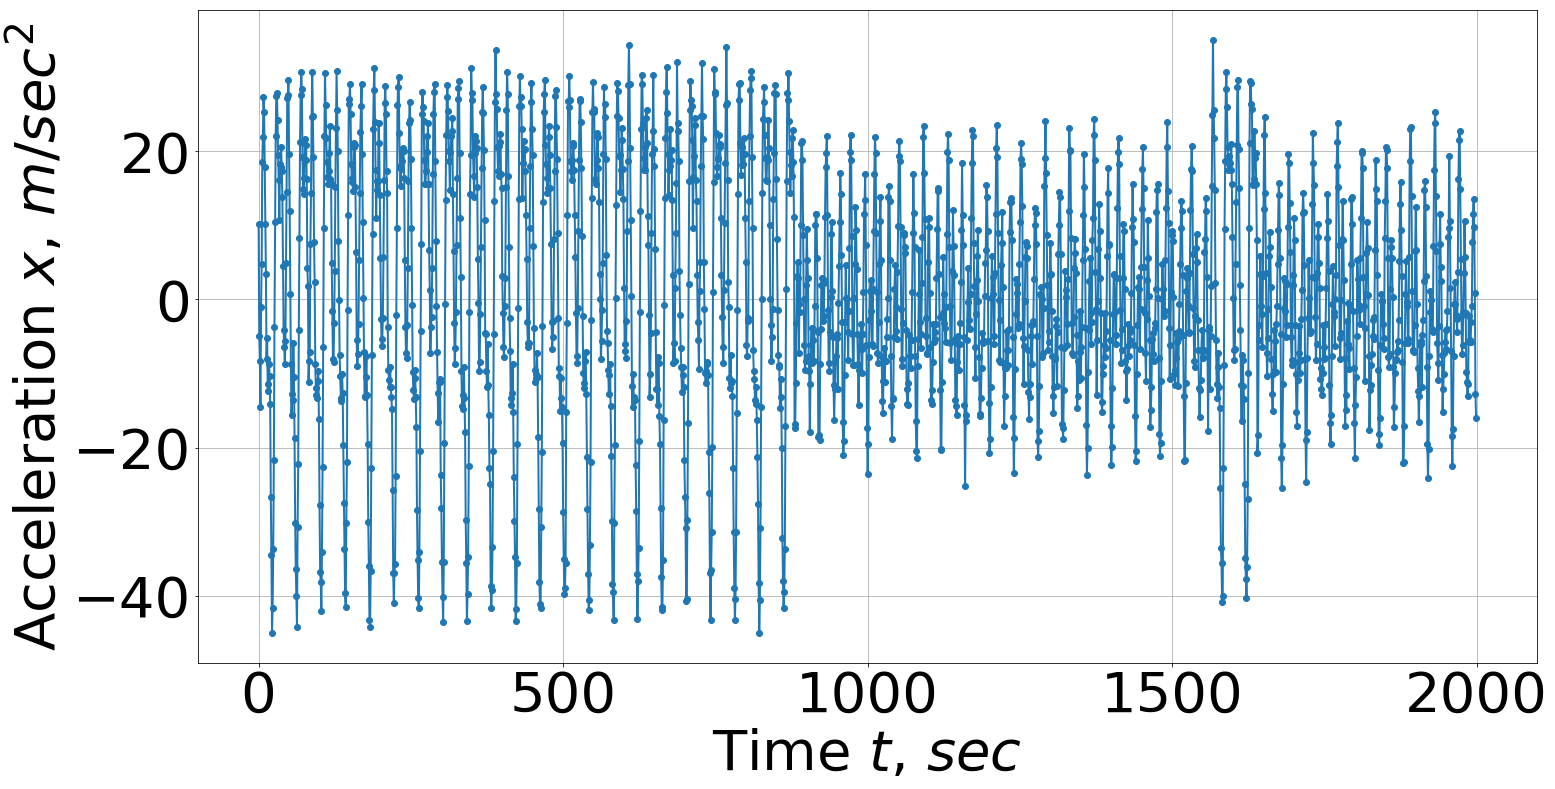
\includegraphics[width=0.5\textwidth]{results/2_patern_series}\label{fig_synthetic_series_2}}
\subfloat[Synthetic 2]
{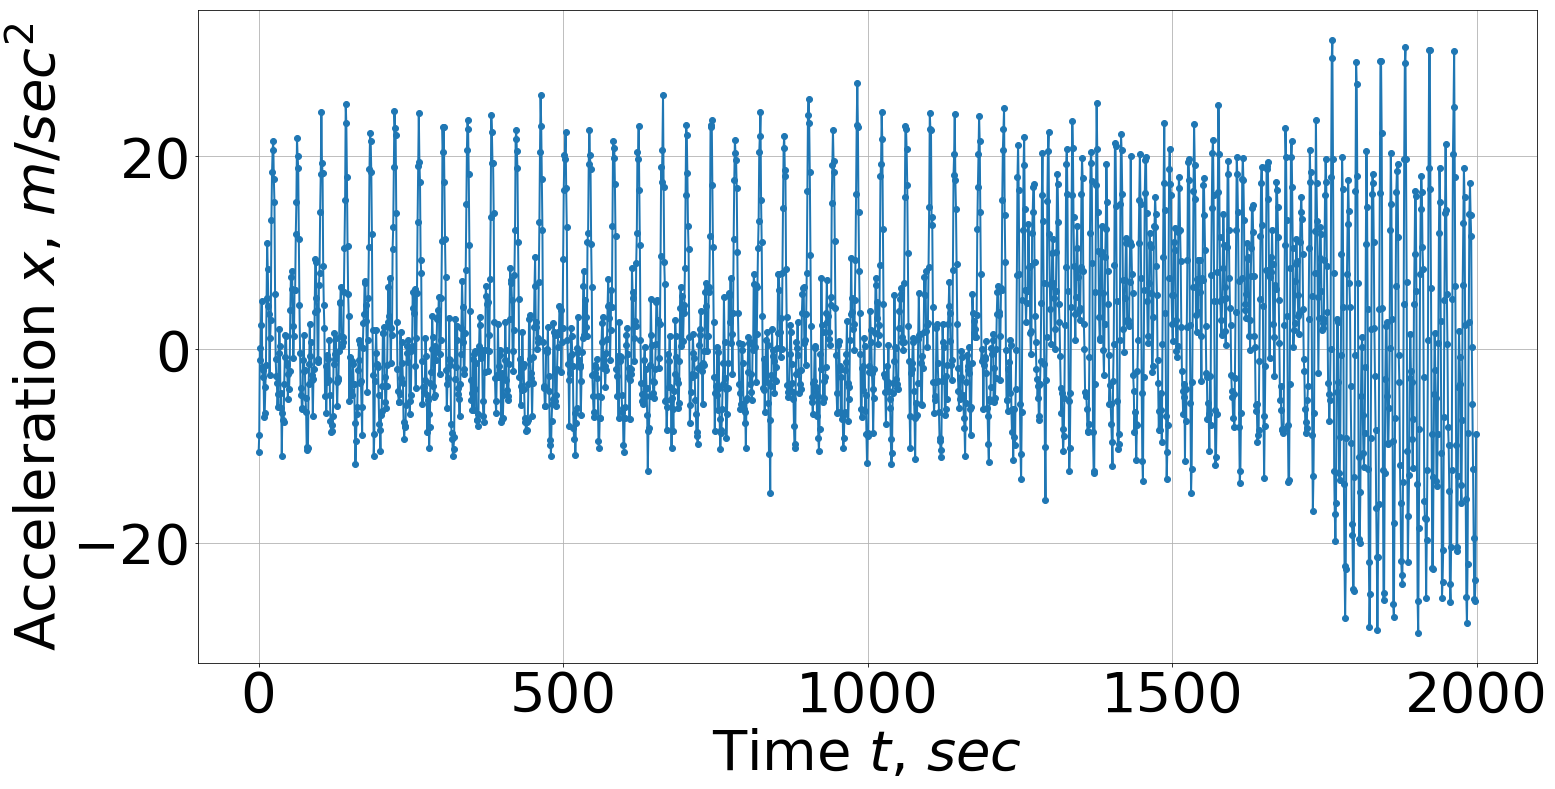
\includegraphics[width=0.5\textwidth]{results/3_patern_series}\label{fig_synthetic_series_3}}\\
\caption{Пример синтетически построенных временных рядов}
\label{fig_synthetic_series}
\end{figure}

\begin{figure}[h!t]\center
\subfloat[Synthetic 1]
{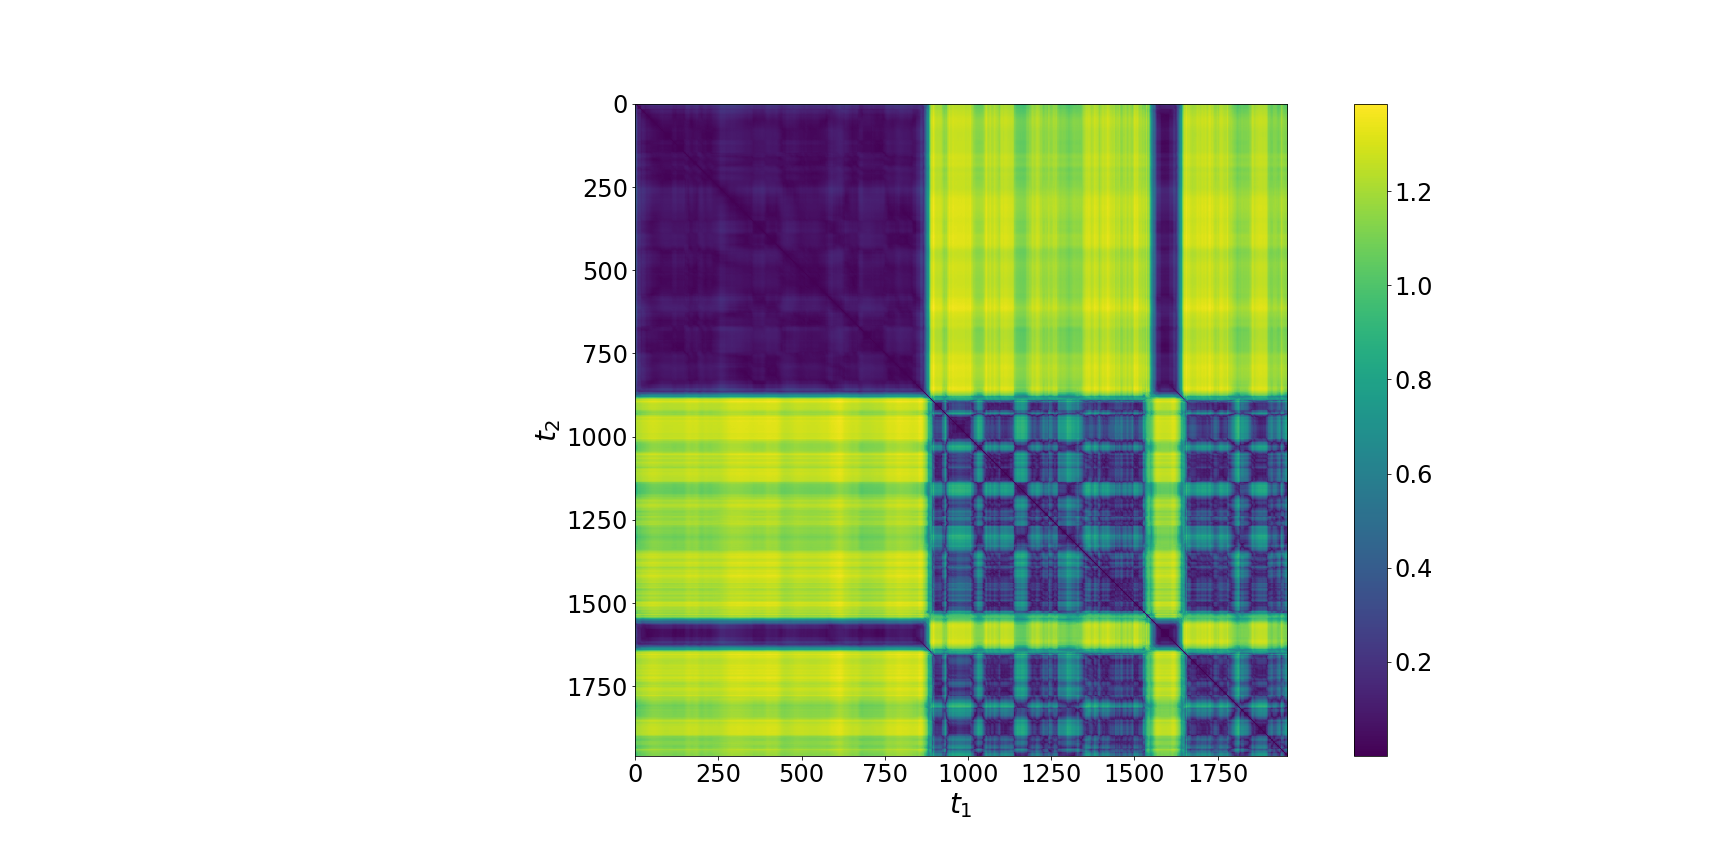
\includegraphics[width=0.5\textwidth]{results/2_patern_full}}
\subfloat[Synthetic 2]
{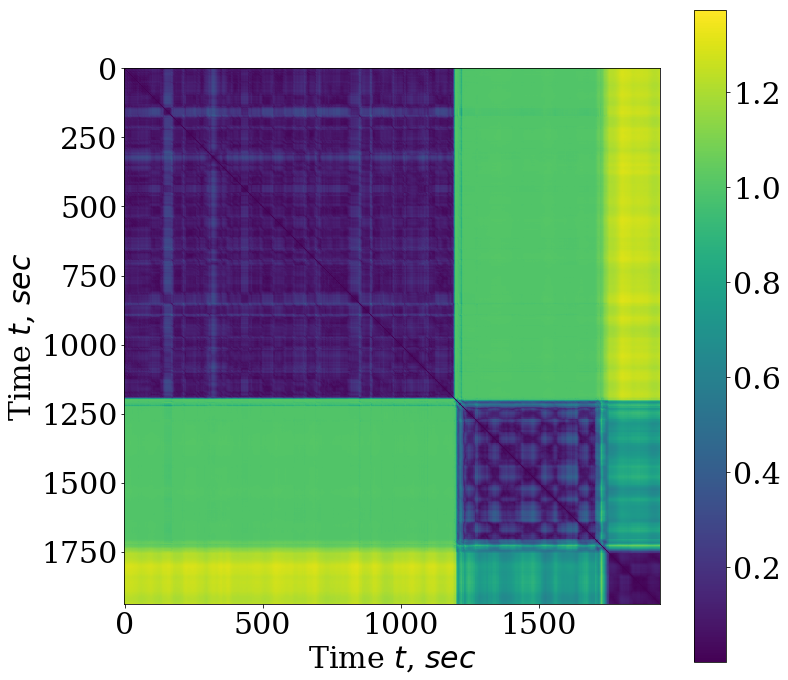
\includegraphics[width=0.5\textwidth]{results/3_patern_full}}\\
\caption{Матрица попарных расстояний $\textbf{M}$ между точками временного ряда}
\label{fig_synthetic_distance}
\end{figure}

\begin{figure}[h!t]\center
\subfloat[Synthetic 1]
{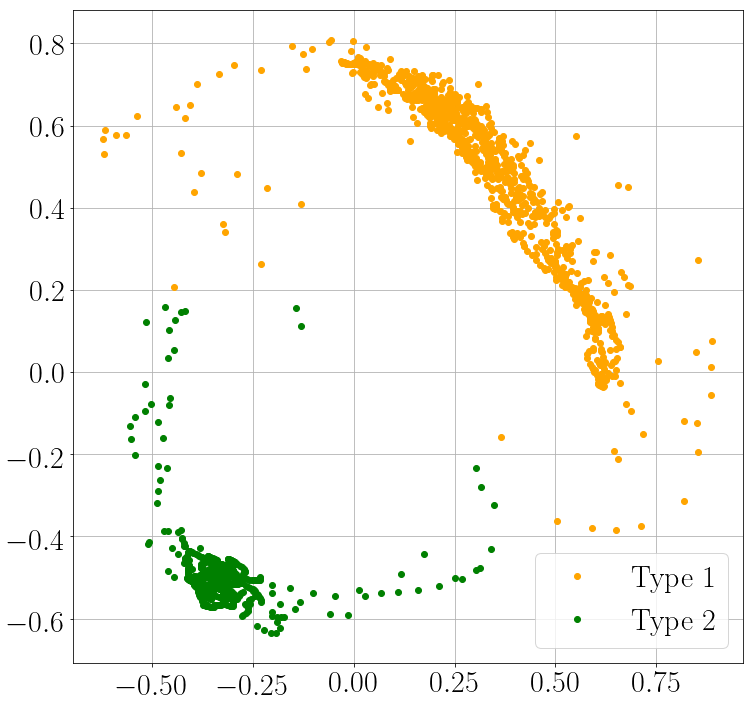
\includegraphics[width=0.5\textwidth]{results/2_patern_2D_vector}}
\subfloat[Synthetic 2]
{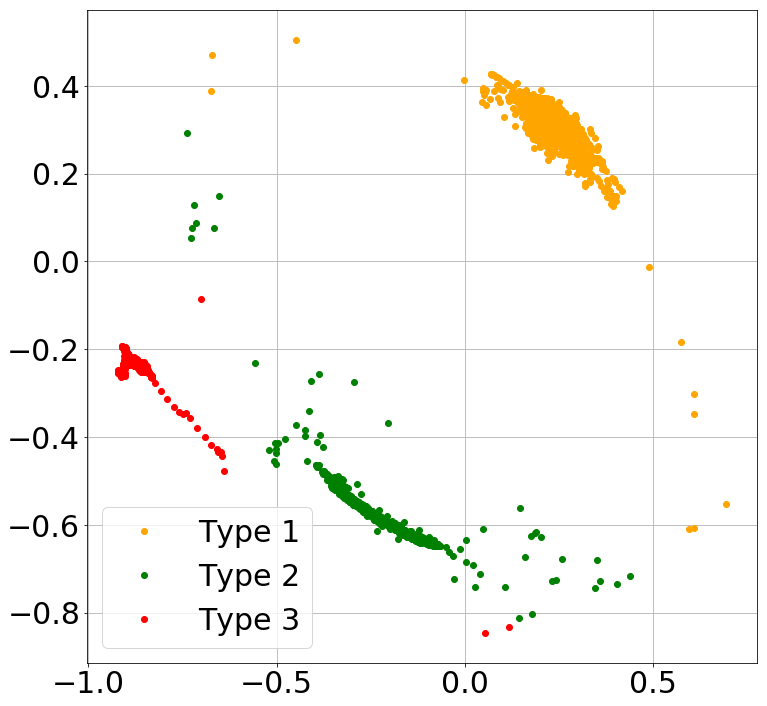
\includegraphics[width=0.5\textwidth]{results/3_patern_2D_vector}}\\
\caption{Проекция точек временного ряда на плоскость при помощи матрицы попарных расстояний $\textbf{M}$}
\label{fig_synthetic_2D}
\end{figure}

\begin{figure}[h!t]\center
\subfloat[Synthetic 1]
{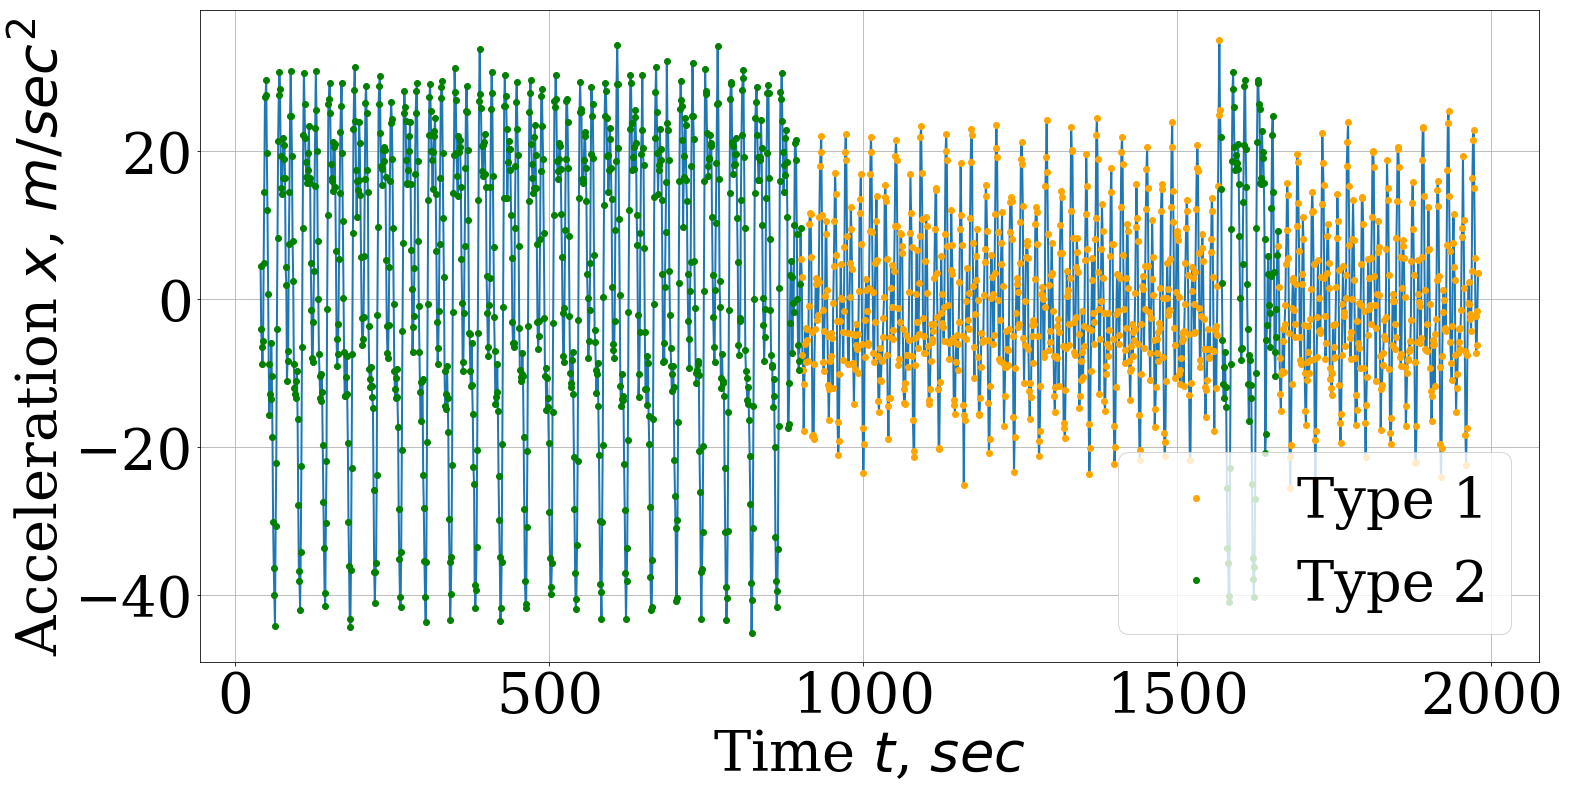
\includegraphics[width=0.5\textwidth]{results/2_patern_claster_vector}}
\subfloat[Synthetic 2]
{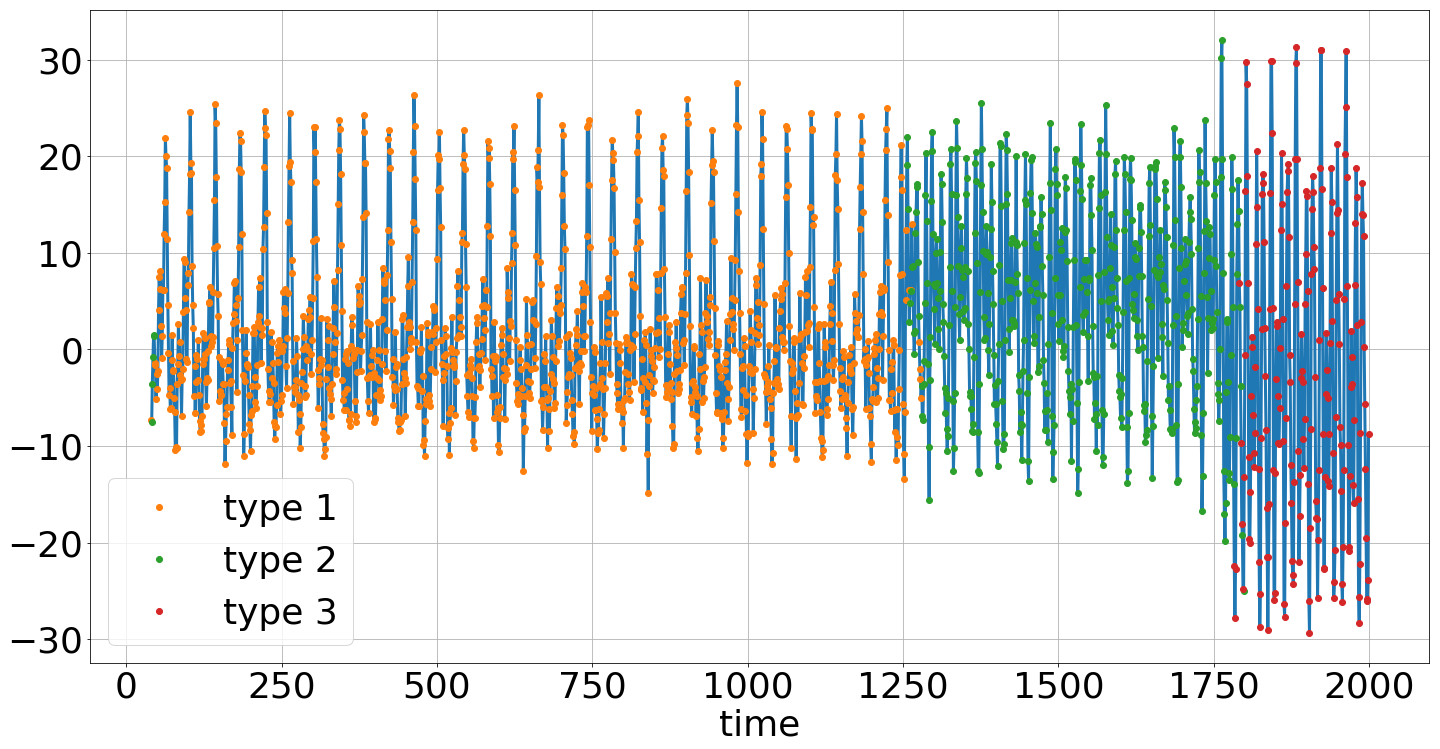
\includegraphics[width=0.5\textwidth]{results/3_patern_claster_vector}}\\
\caption{Кластеризация точек временного ряда}
\label{fig_synthetic_claster}
\end{figure}


\paragraph{Синтетические данные.}


На рис.~\ref{fig_synthetic_series} приведен пример синтетически построенных временных рядов. На рис.~\ref{fig_synthetic_series_2} показан пример ряда в котором количество сигналов $K = 2$, а длина каждого сигнала $T = 20$. На рис.~\ref{fig_synthetic_series_3} показан пример ряда в котором количество сигналов $K = 3$, а длина каждого сигнала $T = 20$. 

На рис.~\ref{fig_synthetic_distance} проиллюстрированы матрицы попарных расстояний $\textbf{M}$ между построены при помощи формулы~(\ref{eq:cl:9}). Используя матрицу попарных расстояний и метод Multidimensional Scaling~\cite{Borg2005} визуальзуализируем точки временного ряда на плоскости. На рис.~\ref{fig_synthetic_2D} показана визуализация точек на плоскости и выполнена их кластеризация при помощи метода KMeans~\cite{Kanungo2000}. Иллюстрация кластеров точек временного ряда продемонстрирована на рис.~\ref{fig_synthetic_claster}.

\begin{figure}[h!t]\center
\subfloat[Physical Motion 1]
{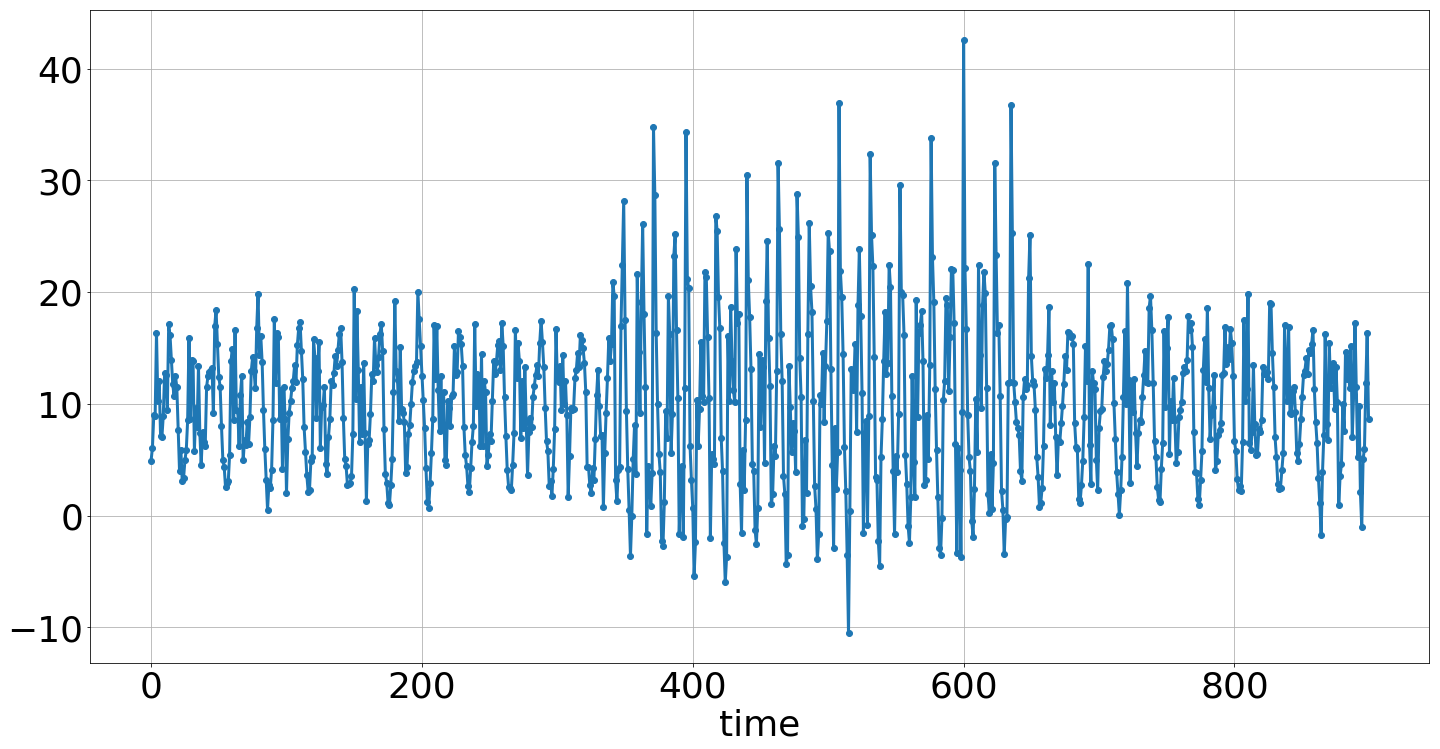
\includegraphics[width=0.5\textwidth]{results/1_real_series}}
\subfloat[Physical Motion 2]
{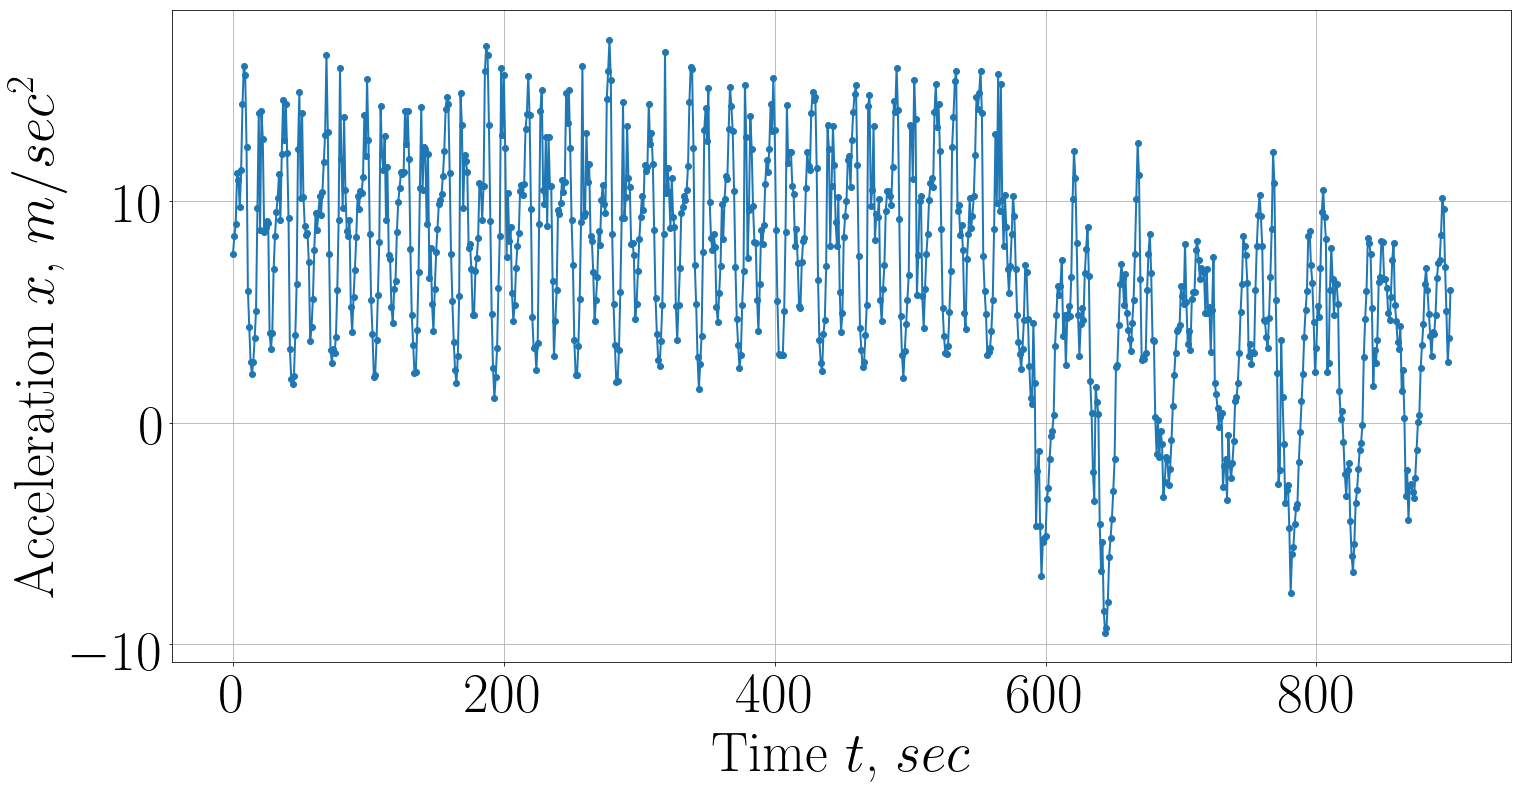
\includegraphics[width=0.5\textwidth]{results/2_real_series}}\\
\caption{Пример синтетически построенных временных рядов}
\label{fig_real_series}
\end{figure}

\begin{figure}[h!t]\center
\subfloat[Physical Motion 1]
{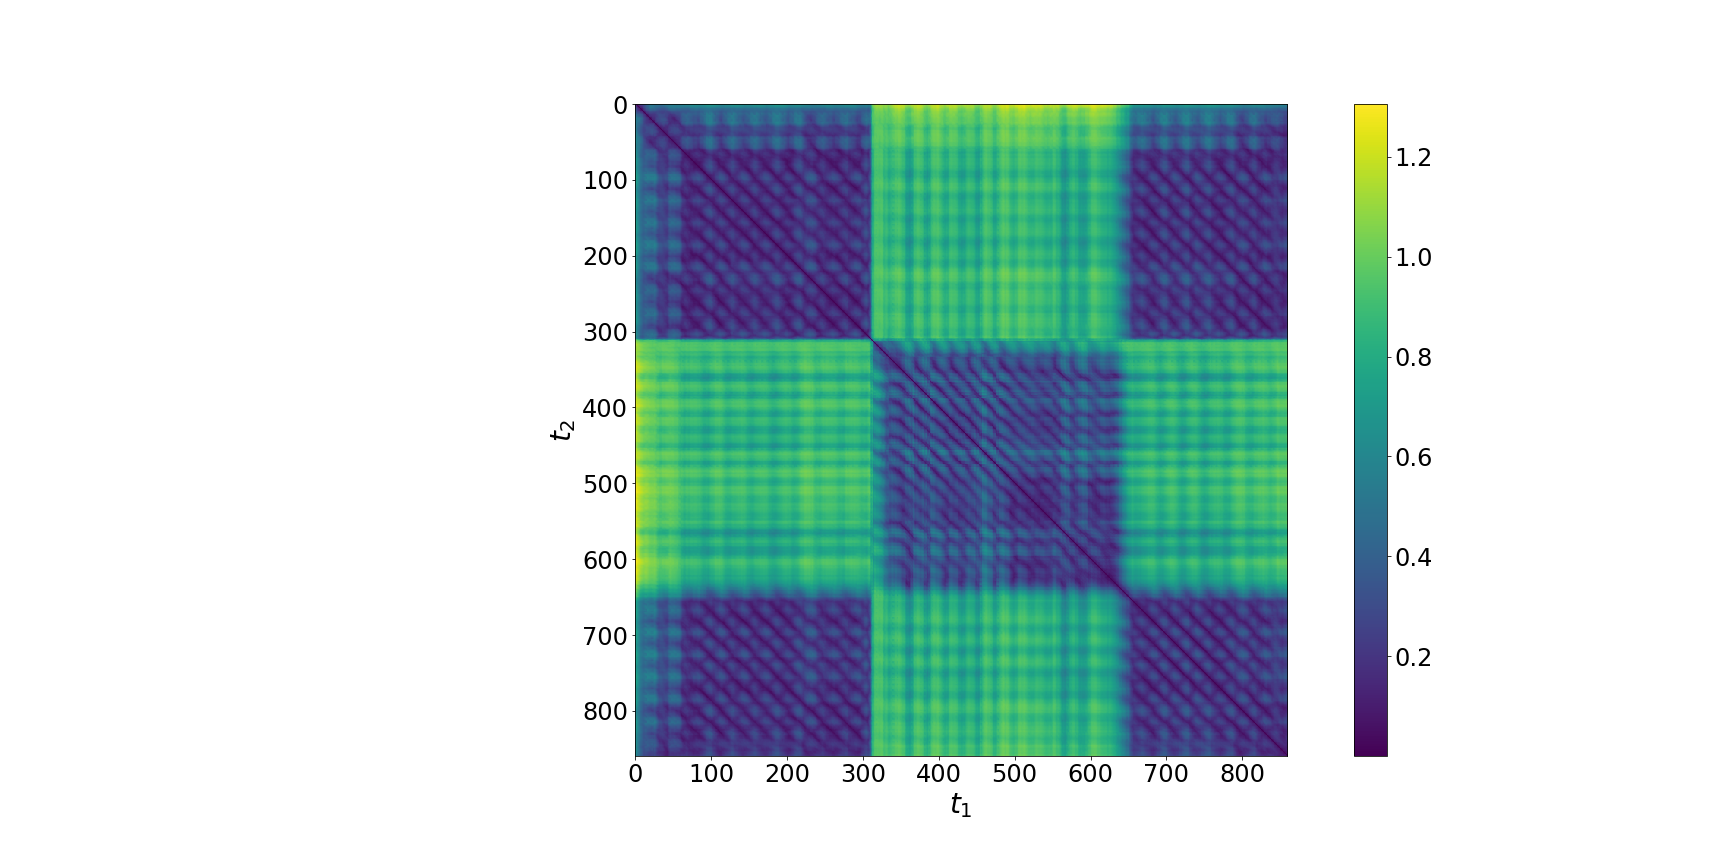
\includegraphics[width=0.5\textwidth]{results/1_real_full}}
\subfloat[Physical Motion 2]
{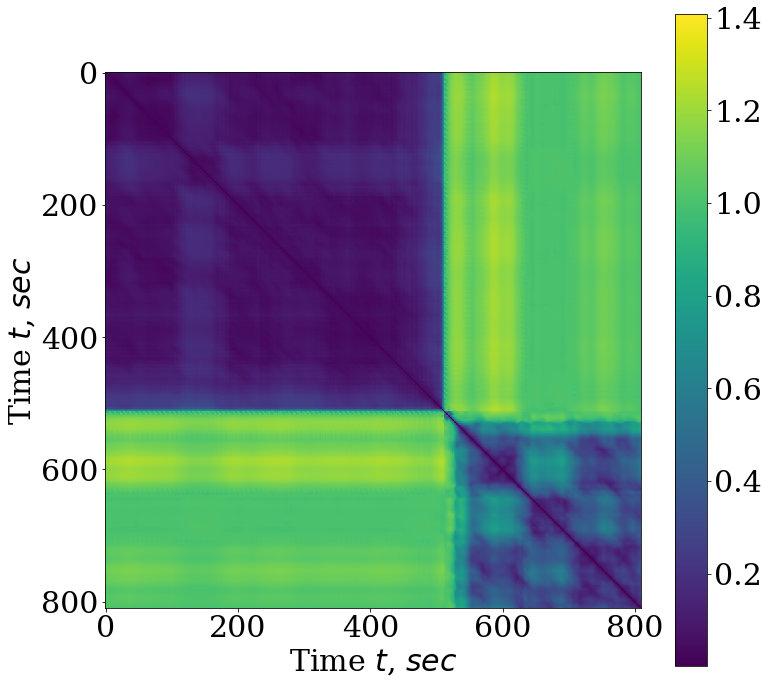
\includegraphics[width=0.5\textwidth]{results/2_real_full}}\\
\caption{Матрица попарных расстояний $\textbf{M}$ между точками временного ряда}
\label{fig_real_distance}
\end{figure}

\begin{figure}[h!t]\center
\subfloat[Physical Motion 1]
{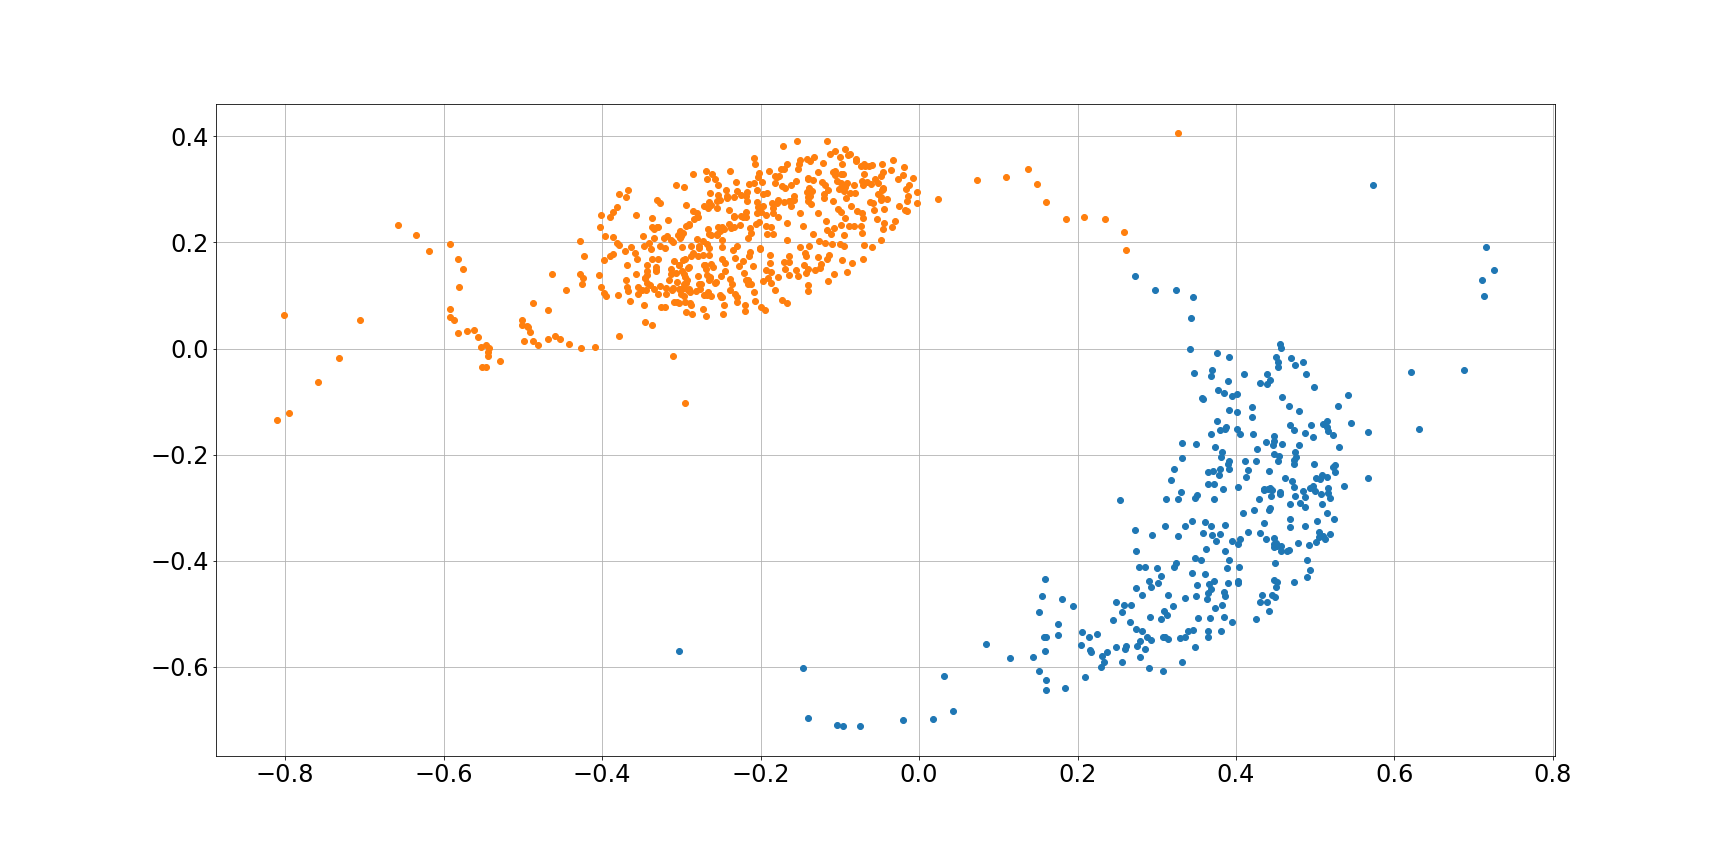
\includegraphics[width=0.5\textwidth]{results/1_real_2D_vector}}
\subfloat[Physical Motion 2]
{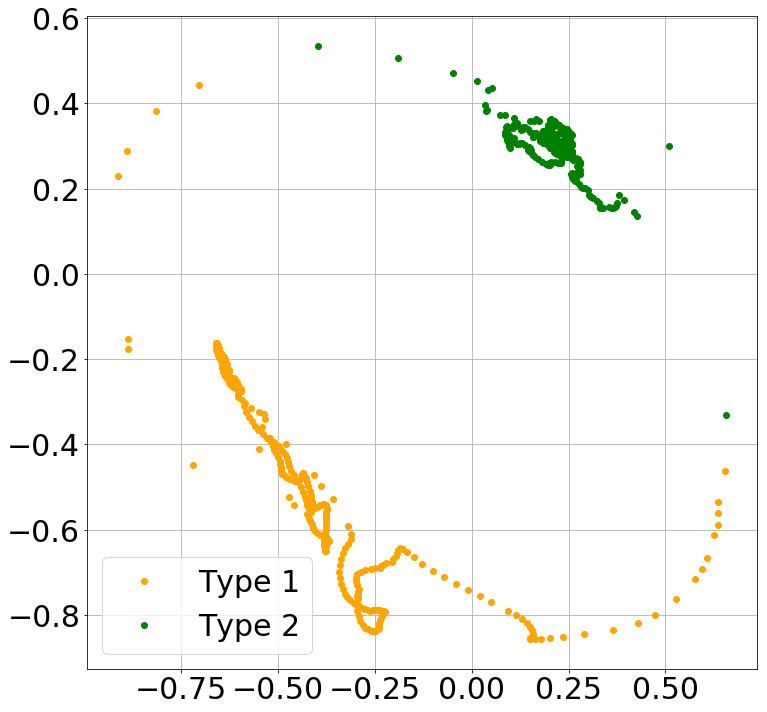
\includegraphics[width=0.5\textwidth]{results/2_real_2D_vector}}\\
\caption{Проекция точек временного на плоскость при помощи матрицы попарных расстояний $\textbf{M}$}
\label{fig_real_2D}
\end{figure}

\begin{figure}[h!t]\center
\subfloat[Physical Motion 1]
{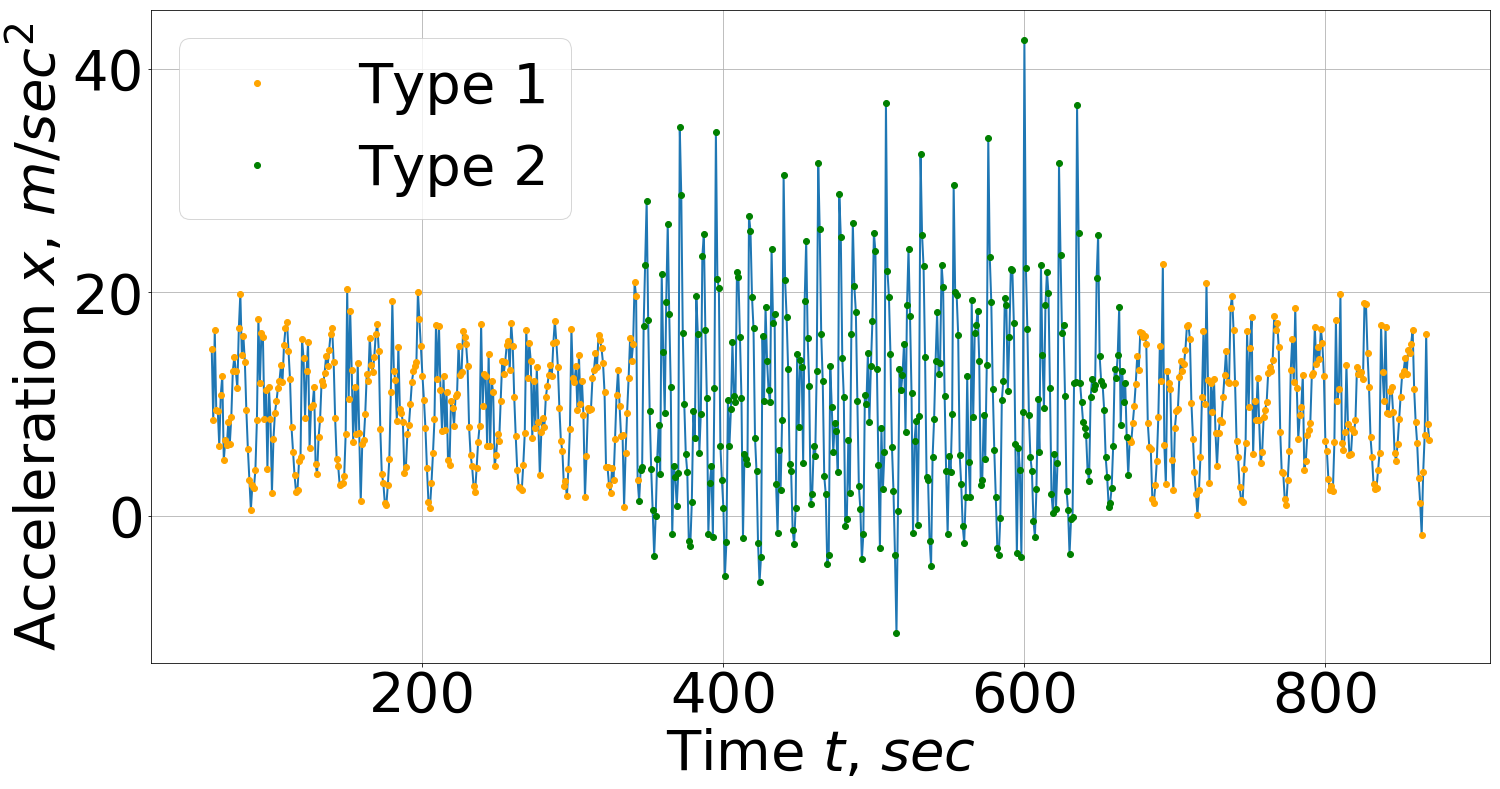
\includegraphics[width=0.5\textwidth]{results/1_real_claster_vector}}
\subfloat[Physical Motion 2]
{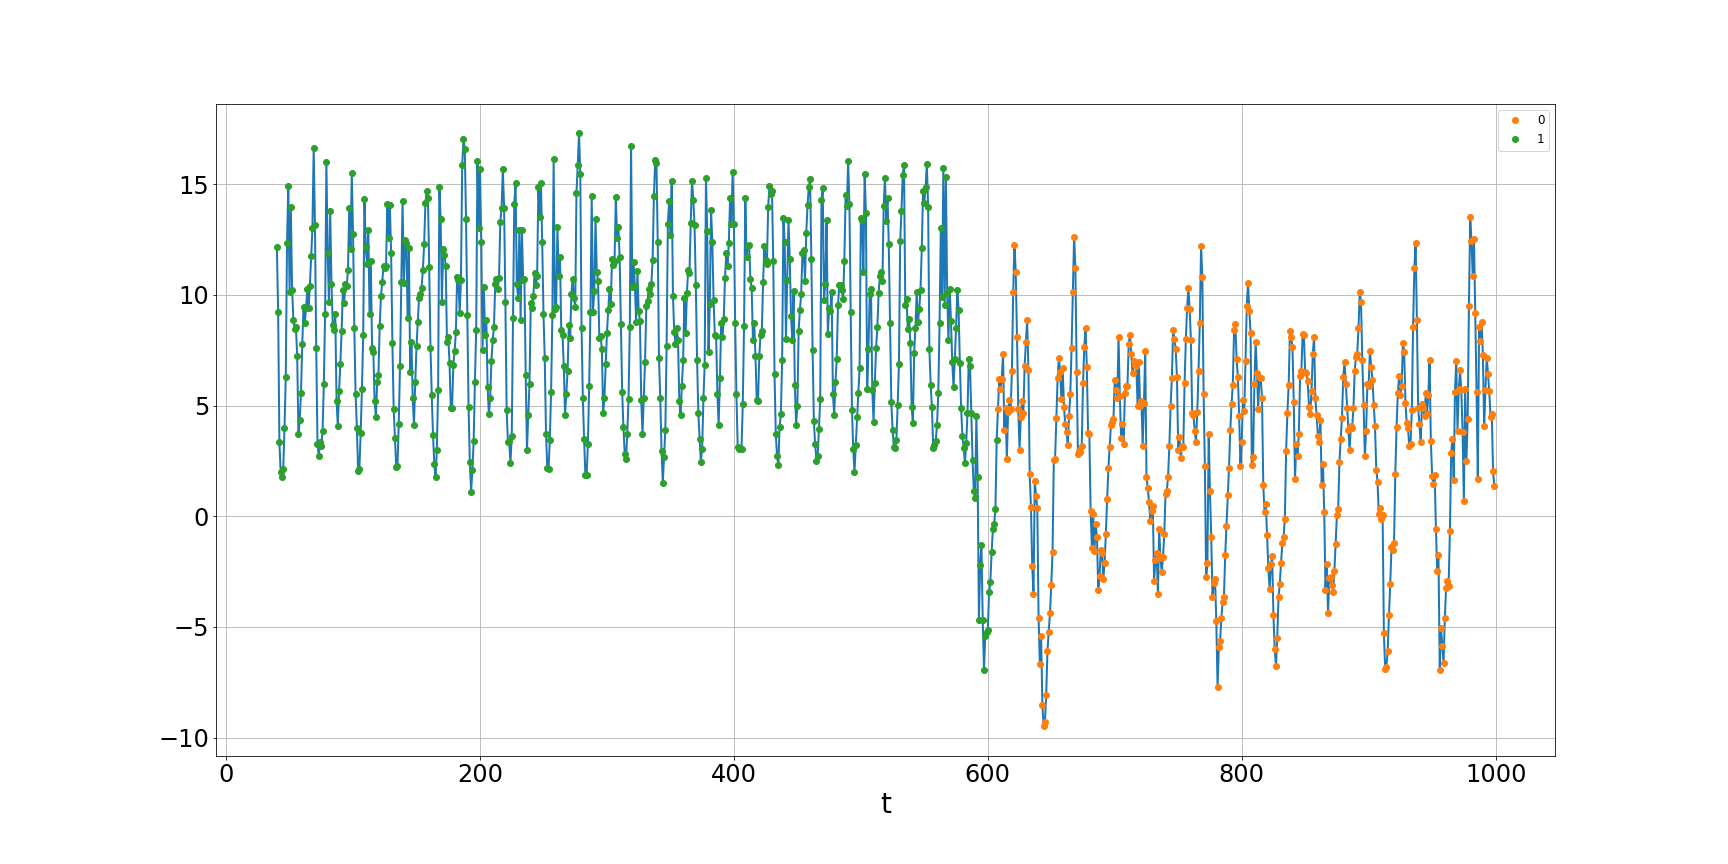
\includegraphics[width=0.5\textwidth]{results/2_real_claster_vector}}\\
\caption{Кластеризация точек временного ряда}
\label{fig_real_claster}
\end{figure}

\paragraph{Реальные данные.}

На рис.~\ref{fig_real_series} приведен пример реальных временных рядов полученных при помощи взятия одной из координат мобильного акселерометра. 



На рис.~\ref{fig_real_distance} проиллюстрированы матрицы попарных расстояний $\textbf{M}$ между построены при помощи формулы~(\ref{eq:cl:9}). Используя матрицу попарных расстояний и метод Multidimensional Scaling~\cite{Borg2005} визуальзуализируем точки временного ряда на плоскости. На рис.~\ref{fig_real_2D} показана визуализация точек на плоскости и выполнена их кластеризация при помощи метода KMeans~\cite{Kanungo2000}. Иллюстрация кластеров точек временного ряда продемонстрирована на рис.~\ref{fig_real_claster}.





\section{Заключение}
\begin{table}[h!t]
\begin{center}
\caption{Результаты работы алгоритма}
\label{table_2}
\begin{tabular}{|c|c|c|c|c|}
\hline
	Ряд & $N$& $K$& $T$& $S$\\
	\hline
	\multicolumn{1}{|l|}{Physical Motion 1}
	& 900& 2& 30& 0.06\\
	\hline
	\multicolumn{1}{|l|}{Physical Motion 2}
	& 1000& 2& 30& 0.03\\
	\hline
	\multicolumn{1}{|l|}{Synthetic 1}
	& 2000& 2& 20& 0.04\\
	\hline
	\multicolumn{1}{|l|}{Synthetic 2}
	& 2000& 3& 20& 0.03\\
\hline

\end{tabular}
\end{center}
\end{table}

В работе рассматривалась задача поиска характерных периодических структур внутри временного ряда. Рассматривался метод основаный на локальном снижение размерности фазового пространства. Был предложен алгоритм поиска характерных сигналов, который основывается на методе главных компонент для локального снижения размерности, а также на использовании некоторой функции расстояния между локальными базисами в каждый момент времени, которые интерпретировались как признакового описание точки временного ряда.

В ходе эксперимента, на реальных показаниях акселерометра, а также на синтетических данных, было показано, что предложенный метод измерение расстояния между базисами хорошо разделяет точки которые принадлежат различным классам, что приводит к хорошей кластеризации объектов. Результаты работы, показаны в таблице~\ref{table_2}.

Предложеный метод имеет ряд недостаткров связаных с большим количеством ограничей на временной ряд. Данные ограничения будут ослаблены в последнующих работах.



\appendix
\section{Теорема (Грабовой 2019)}\label{ProofTheorem1}

\begin{lemma} \label{lem:1} 
Пусть заданы два подпространства $\mathbb{X}, \mathbb{Y} \subset \mathbb{R}^{n}$, которые задаются базисами $\textbf{W}_1$ и  $\textbf{W}_2$, тогда справедливо следующее условие:

\begin{equation}
\label{eq:l1:1}
\begin{aligned}
\max_{\textbf{a} \in \mathbb{X}:~\left|\textbf{a}\right|\leq 1}h_2\left(\textbf{a}\right)
\end{aligned}
\end{equation}
где $h_i\left(\textbf{a}\right)$ является расстоянием от вектора $\textbf{a}$ до пространства заданого базисом $\textbf{W}_i$.
\end{lemma}

\begin{proof}
\begin{equation}
\label{eq:l1:2}
\begin{aligned}
\max_{\textbf{a} \in \mathbb{X}:~\left|\textbf{a}\right|\leq 1}h_2\left(\textbf{a}\right) = \max_{\textbf{a} \in \mathbb{X}:~\left|\textbf{a}\right|\leq 1}\left|\textbf{a}-\sum_{i}\langle \textbf{e}^i_2, \textbf{a} \rangle\textbf{e}^i_2 \right| = \\ 
=\max_{\{\alpha_j\}_{j}:~\sum\alpha_j^2\leq 1}\left|\sum_{j}\alpha_j\textbf{e}^{j}_1-\sum_{i}\langle \textbf{e}^i_2, \sum_{j}\alpha_j\textbf{e}^{j}_1 \rangle\textbf{e}^i_2 \right| =\\
= \max_{\{\alpha_j\}_{j}:~\sum\alpha_j^2\leq 1}\left|\sum_{j}\alpha_j\left(\textbf{e}_3^j - \sum_{i}\langle\textbf{e}_3^j,\textbf{e}_2^i\rangle\textbf{e}_2^i\right)\right|,
\end{aligned}
\end{equation}
где в выражении~(\ref{eq:l1:2}) максимум очевидно достигается на $j$-ом базисном векторе для которого выражение в скобках является максимальным.
\end{proof}




\begin{lemma} \label{lem:2} 
Пусть заданы подпространства $\mathbb{X}, \mathbb{Y}, \mathbb{Z} \subset \mathbb{R}^{n}$, которые задаются базисами $\textbf{W}_1, \textbf{W}_2, \textbf{W}_3$ соответственно, тогда справедливо следующее условие:

\begin{equation}
\label{eq:l2:1}
\begin{aligned}
\max_{\substack{\textbf{x} \in \mathbb{X} \\ \left|\textbf{x}\right|\leq 1}}\min_{\substack{\textbf{y} \in \mathbb{Y} \\ \left|\textbf{y}\right|\leq 1}}||\textbf{x}-\textbf{y}||\leq 
\max_{\substack{\textbf{x} \in \mathbb{X} \\ \left|\textbf{x}\right|\leq 1}}\min_{\substack{\textbf{z} \in \mathbb{Z} \\ \left|\textbf{z}\right|\leq 1}}||\textbf{x}-\textbf{z}|| + 
\max_{\substack{\textbf{z} \in \mathbb{Z} \\ \left|\textbf{z}\right|\leq 1}}\min_{\substack{\textbf{y} \in \mathbb{Y} \\ \left|\textbf{y}\right|\leq 1}}||\textbf{z}-\textbf{y}||.
\end{aligned}
\end{equation}
\end{lemma}

\begin{proof} 
\begin{equation}
\label{eq:l2:2}
\begin{aligned}
\max_{\substack{\textbf{x} \in \mathbb{X} \\ \left|\textbf{x}\right|\leq 1}}\min_{\substack{\textbf{y} \in \mathbb{Y} \\ \left|\textbf{y}\right|\leq 1}}||\textbf{x}-\textbf{y}||\leq
\max_{\substack{\textbf{x} \in \mathbb{X} \\ \left|\textbf{x}\right|\leq 1}}\min_{\substack{\textbf{y} \in \mathbb{Y} \\ \left|\textbf{y}\right|\leq 1}}\left(||\textbf{x}-\textbf{z}|| + ||\textbf{z} - \textbf{y}||\right) = \\
\max_{\substack{\textbf{x} \in \mathbb{X} \\ \left|\textbf{x}\right|\leq 1}}||\textbf{x}-\textbf{z}|| + \min_{\substack{\textbf{y} \in \mathbb{Y} \\ \left|\textbf{y}\right|\leq 1}}||\textbf{z} - \textbf{y}|| = \max_{\substack{\textbf{x} \in \mathbb{X} \\ \left|\textbf{x}\right|\leq 1}}\min_{\substack{\textbf{z} \in \mathbb{Z} \\ \left|\textbf{z}\right|\leq 1}}||\textbf{x}-\textbf{z}|| + \min_{\substack{\textbf{y} \in \mathbb{Y} \\ \left|\textbf{y}\right|\leq 1}}||\textbf{z} - \textbf{y}|| \leq \\
\leq \max_{\substack{\textbf{x} \in \mathbb{X} \\ \left|\textbf{x}\right|\leq 1}}\min_{\substack{\textbf{z} \in \mathbb{Z} \\ \left|\textbf{z}\right|\leq 1}}||\textbf{x}-\textbf{z}|| + 
\max_{\substack{\textbf{z} \in \mathbb{Z} \\ \left|\textbf{z}\right|\leq 1}}\min_{\substack{\textbf{y} \in \mathbb{Y} \\ \left|\textbf{y}\right|\leq 1}}||\textbf{z}-\textbf{y}||.
\end{aligned}
\end{equation}
\end{proof}

\begin{theorem} \label{th:1} 
Пусть задано множество подпространств $\mathbf{W}$ пространства $\mathbb{R}^{n}$, каждое подпространство которого задается базисом, тогда функция расстояния $\rho\left(\textbf{W}_1, \textbf{W}_2\right)$ является метрикой заданой на множестве $\mathbf{W}$:
\begin{equation}
\label{eq:th2:1}
\begin{aligned}
\rho\left(\textbf{W}_1, \textbf{W}_2\right) = \max\left(\max_{\textbf{e}_2 \in \textbf{W}_2} h_{1}\left(\textbf{e}_2\right), \max_{\textbf{e}_1 \in \textbf{W}_1} h_{2}\left(\textbf{e}_1\right)\right),
\end{aligned}
\end{equation}
где $\textbf{e}_i$ это базисный вектор из $\textbf{W}_i$, $h_i\left(\textbf{e}\right)$ является расстоянием от вектора $\textbf{e}$ до пространства заданого базисом $\textbf{W}_i$.
\end{theorem}
\begin{proof}
Для доказательства данной теоремы, нужно показать, что функция $\rho$ удовлетворяет трем свойствам метрики.

Функция $\rho$ удовлетворяет первому свойству метрики:
\begin{equation}
\label{eq:th2:2}
\begin{aligned}
\rho\left(\textbf{W}_1, \textbf{W}_2\right) = 0 \Leftrightarrow \textbf{W}_1 = \textbf{W}_2
\end{aligned}
\end{equation}

Функция $\rho$ удовлетворяет второму свойству метрики:
\begin{equation}
\label{eq:th2:3}
\begin{aligned}
\rho\left(\textbf{W}_1, \textbf{W}_2\right) = \rho\left(\textbf{W}_2, \textbf{W}_1\right)
\end{aligned}
\end{equation}

Докажем, что функция $\rho$ удовлетворяет удовлетворяет неравенству треугольника:
\begin{equation}
\label{eq:th2:4}
\begin{aligned}
\rho\left(\textbf{W}_1, \textbf{W}_2\right) \leq \rho\left(\textbf{W}_1, \textbf{W}_3\right) + \rho\left(\textbf{W}_3, \textbf{W}_2\right)
\end{aligned}
\end{equation}

Для доказательства неравенства треугольника докажем неравенства:
\begin{equation}
\label{eq:th2:5}
\begin{aligned}
\max_{\textbf{e}_1 \in \textbf{W}_1}h_{2}\left(\textbf{e}_1\right) \leq 
\max_{\textbf{e}_1\in \textbf{W}_1}h_{3}\left(\textbf{e}_1\right)+
\max_{\textbf{e}_3 \in \textbf{W}_3}h_{2}\left(\textbf{e}_3\right) \\
\max_{\textbf{e}_2 \in \textbf{W}_2}h_{1}\left(\textbf{e}_2\right) \leq 
\max_{\textbf{e}_2\in \textbf{W}_2}h_{3}\left(\textbf{e}_2\right)+
\max_{\textbf{e}_3 \in \textbf{W}_3}h_{1}\left(\textbf{e}_3\right)
\end{aligned}
\end{equation}

Используя Лемму~\ref{lem:1} доказательство неравенства (\ref{eq:th2:5}) сводится к доказательства неравенства:
\begin{equation}
\label{eq:th2:6}
\begin{aligned}
\max_{\substack{\textbf{a} \in \textbf{W}_1 \\ \left|\textbf{a}\right| \leq 1}}h_{2}\left(\textbf{a}\right) \leq 
\max_{\substack{\textbf{a} \in \textbf{W}_1 \\ \left|\textbf{a}\right| \leq 1}}h_{3}\left(\textbf{a}\right)+
\max_{\substack{\textbf{c} \in \textbf{W}_3 \\ \left|\textbf{c}\right| \leq 1}}h_{2}\left(\textbf{c}\right),
\end{aligned}
\end{equation}
где $\textbf{a}, \textbf{c}$ произвольные элементы из соответствующих подпространств. 

Подставив в выражение~(\ref{eq:th2:6}) выражение для $h_i\left(\textbf{a}\right)$, получаем следующее неравенство:
\begin{equation}
\label{eq:th2:7}
\begin{aligned}
\max_{\substack{\textbf{a} \in \textbf{W}_1 \\ \left|\textbf{a}\right| \leq 1}} \min_{\substack{\textbf{b} \in \textbf{W}_2 \\ \left|\textbf{b}\right| \leq 1}}||\textbf{a} - \textbf{b}|| \leq 
\max_{\substack{\textbf{a} \in \textbf{W}_1 \\ \left|\textbf{a}\right| \leq 1}} \min_{\substack{\textbf{c} \in \textbf{W}_3 \\ \left|\textbf{b}\right| \leq 1}}||\textbf{a} - \textbf{c}||+
\max_{\substack{\textbf{c} \in \textbf{W}_3 \\ \left|\textbf{c}\right| \leq 1}} \min_{\substack{\textbf{b} \in \textbf{W}_2 \\ \left|\textbf{b}\right| \leq 1}}||\textbf{c} - \textbf{b}||.
\end{aligned}
\end{equation}

Неравенство~(\ref{eq:th2:7}) следует из Леммы~\ref{lem:2}. Из выполнения неравенства~(\ref{eq:th2:7}) следует выполнение неравенств~(\ref{eq:th2:5}).
Докажем неравенство треугольника~(\ref{eq:th2:4}) используя неравенства~(\ref{eq:th2:5}). Для удобства введем следующие обозначения:
\begin{equation}
\label{eq:th2:8}
\begin{aligned}
\max_{\textbf{e}_i \in \textbf{W}_i} h_{\textbf{W}_j}\left(\textbf{e}_i\right) = h_{i}^{j}.
\end{aligned}
\end{equation}

Из истинности неравенства~(\ref{eq:th2:7}) в обозначениях~(\ref{eq:th2:8}) следует истинность следующих неравенств:
 
\begin{equation}
\label{eq:th2:9}
\begin{aligned}
\quad h_{1}^{2} \leq h_{1}^{3} + h_{3}^{2} \leq \max\left(h_{1}^{3}, h_{3}^{1}\right) + \max\left(h_{3}^{2}, h_{2}^{3}\right)\\
\quad h_{2}^{1} \leq h_{2}^{3} + h_{3}^{1} \leq \max\left(h_{2}^{3}, h_{3}^{2}\right) + \max\left(h_{3}^{1}, h_{1}^{3}\right)\\
\end{aligned}
\end{equation}

Из уравнения~(\ref{eq:th2:9}) следует выполнение неравенства:
\begin{equation}
\label{eq:th2:10}
\begin{aligned}
\max\left(h_{1}^{2}, h_{2}^{1}\right) \leq  \max\left(h_{1}^{3}, h_{3}^{1}\right) + \max\left(h_{3}^{2}, h_{2}^{3}\right)\\
\end{aligned}
\end{equation}

Доказательство неравенства~(\ref{eq:th2:10}) указывает на выполнение неравенства треугольника для функции $\rho$, что завершает доказательство того, что $\rho$ является метрикой.

\end{proof}

\begin{thebibliography}{99}
	\bibitem{cinar2018}
	\textit{Y. G. Cinar and H. Mirisaee} Period-aware content attention RNNs for time series forecasting with missing values~// Neurocomputing, 2018. Vol. 312. P. 177--186.
	
	\bibitem{Ivkin2015}
	\textit{И. П. Ивкин,  М. П. Кузнецов} Алгоритм классификации временных рядов акселерометра по комбинированному признаковому описанию.~// Машинное обучение и анализ данных, 2015.
	
	\bibitem{Katrutsa2015}
	\textit{V. V. Strijov, A. M. Katrutsa} Stresstes procedures for features selection algorithms.~// Schemometrics and Intelligent Laboratory System, 2015.
	
	\bibitem{Borg2005}
	\textit{I. Borg, P. J. F. Groenen} Modern Multidimensional Scaling. --- New York: Springer, 2005. 540 p.
	
	\bibitem{Kanungo2000}
	\textit{T. Kanungo, D. M. Mount et al} An Efficient k-Means Clustering Algorithm: Analysis and Implementation. 2000.
	
	\bibitem{Shiglavsi1997}
	\textit{Д. Л. Данилова, А. А. Жигловский} Главные компоненты временных рядов: метод "Гусеница". --- Санкт-Петербурскиий университет, 1997.
	
	\bibitem{Ignatov2015}
	\textit{A. D. Ignatov, V. V. Strijov} Human activity recognition using quasiperiodic time series collected from a single tri-axial accelerometer.~// Multimedial Tools and Applications, 2015.
	
	\bibitem{Olivares2012}
	\textit{A. Olivares, J. Ramirez, J. M. Gorris, G. Olivares, M. Damas} Detec- tion of (in)activity periods in human body motion using inertial sensors: A comparative study.~// Sensors, 12(5):5791–5814, 2012.

	
\end{thebibliography}

\end{document}

